\section{Bit of  Differential Geometry: Dayuum!!}
Let us look into a bit of differential geometry which is a formal way of treating this tensor thingy. We will try to be as intuitive and non-rigorous as possible (and thus increasing our chances of making a mathematician crazy!) but yeah, we will try to be rigorous enough so that I am satisfied.
\subsection{Some prior things}
Before touching manifolds, let us define what an abstract topological space is, since manifolds are special case of topological spaces. Basically, a topological space is a set $(X, \tau )$ where $\tau \subset \mathcal{P}$ is a collection of subsets of $X$ such that:
\begin{itemize}
    \item $\emptyset, X \in \tau$.
    \item $U_\alpha \in \tau \implies \bigcup \limits_{\alpha\in J} U_\alpha \in \tau$  (closed under arbitrary union).
    \item $U_i \in \tau \implies \bigcap \limits_{i=1}^n U_i \in \tau$  (closed under finite intersection)\footnote{Here $\alpha$ index is used when we want the indexing set $J$ (indexing set means the set from where the incides to denote the elements of the set are taken from) to be arbitrary, meaning that the set $\{U_\alpha\}$ can be finite, countable or uncountable. On the other hand, index $i$ is mostly used when the indexing set is finite.}.
\end{itemize}
Well well, this does not look anything like coffee cup and donut which most people associate topology with. That is a case of \textit{homeomorphism} which will be discussed later (hopefully). However, for now let us proceed. The sets belonging to $\tau$ are called \textbf{open sets}. We define a \textbf{closed set} as a set whose complement is open. There are umpteen other definitions like \textbf{closure, boundary, interior, neighbourhood}, etc. Let define few of them \emoji{loudly-crying-face}. 
\begin{itemize}
    \item \textit{Closure} of a set $A$ is the smallest closed set containing $A$ and is denoted by $\overline{A}$.
    \item \textit{Interior} of a set $A$ is the largest open set contained in $A$ and is denoted by $\text{int}(A)$.
    \item \textit{Boundary} of a set $A$ is the set of points which are neither in the interior nor in the exterior of $A$ and is denoted by $\partial A$.
    \item If $p\in X$, then a \textit{neighbourhood} of $p$ is a set $N$ such that there exists an open set $U\in \tau$ with $p\in U\subseteq N$.
\begin{figure}[H]
      \centering
      

\tikzset{every picture/.style={line width=0.75pt}} %set default line width to 0.75pt        

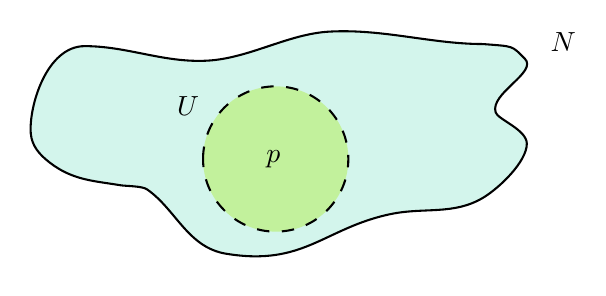
\begin{tikzpicture}[x=0.75pt,y=0.75pt,yscale=-1,xscale=1]
%uncomment if require: \path (0,203); %set diagram left start at 0, and has height of 203

%Curve Lines [id:da28281619681811754] 
\draw [fill={rgb, 255:red, 211; green, 245; blue, 236 }  ,fill opacity=1 ][line width=0.75] [line join = round][line cap = round]   (264,41.63) .. controls (239.07,41.63) and (216.02,34.24) .. (190,35.63) .. controls (169.94,36.71) and (151.25,48.57) .. (131,49.63) .. controls (109.98,50.74) and (92.57,42.63) .. (72,42.63) .. controls (53.59,42.63) and (45.01,71.73) .. (46,84.63) .. controls (46.47,90.7) and (50.18,94.88) .. (55,98.63) .. controls (66.08,107.25) and (76.24,107.51) .. (89,109.63) .. controls (91.95,110.13) and (99.58,109.96) .. (102,111.63) .. controls (115.88,121.24) and (121.56,139.56) .. (140,142.63) .. controls (177.55,148.89) and (187.14,130.46) .. (219,123.63) .. controls (235.52,120.09) and (249.69,124.22) .. (264,115.63) .. controls (271.71,111.01) and (285,98.32) .. (285,89.63) .. controls (285,82.9) and (271.1,77.94) .. (270,74.63) .. controls (266.91,65.36) and (290.59,55.22) .. (284,48.63) .. controls (277.54,42.17) and (279,42.85) .. (264,41.63) -- cycle ;
%Shape: Circle [id:dp001327175657310109] 
\draw  [fill={rgb, 255:red, 194; green, 241; blue, 156 }  ,fill opacity=1 ][dash pattern={on 4.5pt off 4.5pt}] (129,97) .. controls (129,77.67) and (144.67,62) .. (164,62) .. controls (183.33,62) and (199,77.67) .. (199,97) .. controls (199,116.33) and (183.33,132) .. (164,132) .. controls (144.67,132) and (129,116.33) .. (129,97) -- cycle ;

% Text Node
\draw (158,91.4) node [anchor=north west][inner sep=0.75pt]    {$p$};
% Text Node
\draw (115,65.4) node [anchor=north west][inner sep=0.75pt]    {$U$};
% Text Node
\draw (295,34.4) node [anchor=north west][inner sep=0.75pt]    {$N$};


\end{tikzpicture}

      \caption{Neighbourhood of a point $p$ in  $X$}
\end{figure}
          \item \textit{Hausdorff Space}: A topological space is called Hausdorff if for any two distinct points $x,y\in X$, there exist open sets $U,V\in \tau$ such that $x\in U, y\in V$ and $U\cap V = \emptyset$. 
    \begin{figure}[H]
      \centering
      

\tikzset{every picture/.style={line width=0.75pt}} %set default line width to 0.75pt        

\begin{tikzpicture}[x=0.75pt,y=0.75pt,yscale=-1,xscale=1]
%uncomment if require: \path (0,203); %set diagram left start at 0, and has height of 203

%Shape: Circle [id:dp44753041237162206] 
\draw  [dash pattern={on 4.5pt off 4.5pt}] (129,97) .. controls (129,77.67) and (144.67,62) .. (164,62) .. controls (183.33,62) and (199,77.67) .. (199,97) .. controls (199,116.33) and (183.33,132) .. (164,132) .. controls (144.67,132) and (129,116.33) .. (129,97) -- cycle ;
%Shape: Circle [id:dp09577026242923825] 
\draw  [dash pattern={on 4.5pt off 4.5pt}] (230,98.5) .. controls (230,75.03) and (249.03,56) .. (272.5,56) .. controls (295.97,56) and (315,75.03) .. (315,98.5) .. controls (315,121.97) and (295.97,141) .. (272.5,141) .. controls (249.03,141) and (230,121.97) .. (230,98.5) -- cycle ;

% Text Node
\draw (159,92.4) node [anchor=north west][inner sep=0.75pt]    {$x$};
% Text Node
\draw (267,92.4) node [anchor=north west][inner sep=0.75pt]    {$y$};
% Text Node
\draw (113,56.4) node [anchor=north west][inner sep=0.75pt]    {$U$};
% Text Node
\draw (307,47.4) node [anchor=north west][inner sep=0.75pt]    {$V$};


\end{tikzpicture}

      \caption{A \textbf{Hausdorff Space}, where the points $x$ and $y$ are separated by the open sets $U$ and $V$.}
    \end{figure}
    \item \textit{Topological Continuity}: A function $f: X \to Y$ between two topological spaces is said to be continuous if for every open set $V \in \tau_Y$, the preimage $f^{-1}(V)\footnote{The preimage of a set $Y$ under the function $f$ is defined as $f^{-1}(Y) = \{x|f(x)\in Y\}$. Note that this has nothing to do with inverse of a function (sadly we use the same notation)} \in \tau_X$ is open in $X$.
    \item \textit{homeomorphism}: A homeomorphism is a bijective function $f: X\to Y$ between two topological spaces such that both $f$ and its inverse $f^{-1}$ are continuous. If such a function exists, we say that the two spaces are \textbf{homeomorphic} and we write $X\cong Y$.
  \end{itemize}
\subsection{Manifolds}
Let us see some pictures. 
\begin{figure}[H]
  \centering

  \begin{subfigure}[b]{0.3\textwidth}
    \centering
    

\tikzset{every picture/.style={line width=0.75pt}} %set default line width to 0.75pt        

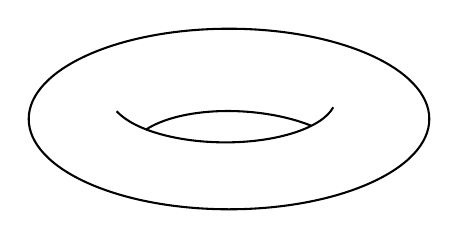
\begin{tikzpicture}[x=0.75pt,y=0.75pt,yscale=-1,xscale=1]
%uncomment if require: \path (0,300); %set diagram left start at 0, and has height of 300

%Shape: Ellipse [id:dp22801969143067424] 
\draw   (104,164.5) .. controls (104,140.48) and (147.2,121) .. (200.5,121) .. controls (253.8,121) and (297,140.48) .. (297,164.5) .. controls (297,188.52) and (253.8,208) .. (200.5,208) .. controls (147.2,208) and (104,188.52) .. (104,164.5) -- cycle ;
%Shape: Arc [id:dp10077529814620967] 
\draw  [draw opacity=0] (250.72,158.87) .. controls (245.28,168.82) and (223.36,176.06) .. (197.24,175.75) .. controls (173.88,175.48) and (154.02,169.25) .. (146.36,160.73) -- (197.5,153.5) -- cycle ; \draw   (250.72,158.87) .. controls (245.28,168.82) and (223.36,176.06) .. (197.24,175.75) .. controls (173.88,175.48) and (154.02,169.25) .. (146.36,160.73) ;  
%Shape: Arc [id:dp345385029103655] 
\draw  [draw opacity=0] (160.45,169.6) .. controls (170.37,163.16) and (188.19,159.59) .. (208.22,160.93) .. controls (220.26,161.74) and (231.27,164.2) .. (240.09,167.72) -- (206.61,184.82) -- cycle ; \draw   (160.45,169.6) .. controls (170.37,163.16) and (188.19,159.59) .. (208.22,160.93) .. controls (220.26,161.74) and (231.27,164.2) .. (240.09,167.72) ;  





\end{tikzpicture}

    \caption{Torus (yeah, donut came atlast!)}
  \end{subfigure}
  \hfill
  \begin{subfigure}[b]{0.3\textwidth}
    \centering
    

\tikzset{every picture/.style={line width=0.75pt}} %set default line width to 0.75pt        

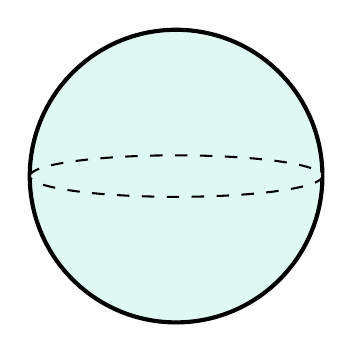
\begin{tikzpicture}[x=0.75pt,y=0.75pt,yscale=-1,xscale=1]
%uncomment if require: \path (0,300); %set diagram left start at 0, and has height of 300

%Shape: Circle [id:dp5828809729635696] 
\draw  [fill={rgb, 255:red, 223; green, 248; blue, 241 }  ,fill opacity=1 ][line width=1.5]  (161,152.5) .. controls (161,113.56) and (192.56,82) .. (231.5,82) .. controls (270.44,82) and (302,113.56) .. (302,152.5) .. controls (302,191.44) and (270.44,223) .. (231.5,223) .. controls (192.56,223) and (161,191.44) .. (161,152.5) -- cycle ;
%Shape: Ellipse [id:dp9903216585683989] 
\draw  [fill={rgb, 255:red, 223; green, 248; blue, 241 }  ,fill opacity=1 ][dash pattern={on 4.5pt off 4.5pt}] (161,152.5) .. controls (161,146.98) and (192.56,142.5) .. (231.5,142.5) .. controls (270.44,142.5) and (302,146.98) .. (302,152.5) .. controls (302,158.02) and (270.44,162.5) .. (231.5,162.5) .. controls (192.56,162.5) and (161,158.02) .. (161,152.5) -- cycle ;




\end{tikzpicture}

    \caption{Sphere (like yo mama)}
  \end{subfigure}
  \hfill
  \begin{subfigure}[b]{0.3\textwidth}
    \centering
    

\tikzset{every picture/.style={line width=0.75pt}} %set default line width to 0.75pt        

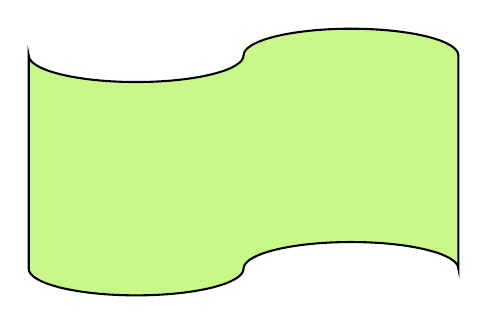
\begin{tikzpicture}[x=0.75pt,y=0.75pt,yscale=-1,xscale=1]
%uncomment if require: \path (0,300); %set diagram left start at 0, and has height of 300

%Flowchart: Punched Tape [id:dp25700721970086793] 
\draw  [fill={rgb, 255:red, 201; green, 248; blue, 137 }  ,fill opacity=1 ] (155,67.85) .. controls (155,74.94) and (178.17,80.69) .. (206.75,80.69) .. controls (235.33,80.69) and (258.5,74.94) .. (258.5,67.85) .. controls (258.5,60.75) and (281.67,55) .. (310.25,55) .. controls (338.83,55) and (362,60.75) .. (362,67.85) -- (362,170.62) .. controls (362,163.52) and (338.83,157.77) .. (310.25,157.77) .. controls (281.67,157.77) and (258.5,163.52) .. (258.5,170.62) .. controls (258.5,177.72) and (235.33,183.47) .. (206.75,183.47) .. controls (178.17,183.47) and (155,177.72) .. (155,170.62) -- cycle ;




\end{tikzpicture}

    \caption{A Waving Flag perhaps?}
  \end{subfigure}

  \caption{\textbf{What's common in all these?}}
\end{figure}
\noindent
So, what is common in all these pictures? Note that they all look very different from each other but if we really ZOOM in \emoji{mag-right} we can see that each of them look alike, like a \textit{flat plane}. Well, the road ahead of us looks flat but the road is on the freaking Earth which is, let's say to a physicist's satisfaction, a sphere. So, we can say that all of these things look `locally' like the flat plane $\mathbb{R}^2$. This is essentially the idea behind a \textbf{manifold}, things which look locally Euclidean. 
\subsection{Tangent Spaces}
\subsection{Differential Forms}
% \textit{Definition.} Suppose $C\subset \mathbb{R}^2$ be a curve and let $p\in C$ is a point. The tangent space to $C$ at $p$ is the set of all vectors tangent to $C$ at $p$ and is denoted by $T_pC$. 